\fontsize{14}{16pt}\selectfont
\chapter{\\\hspace{-6mm}Результаты симуляции}
\label{cha:appendix2}

%Lab1
\begin{figure}[h!]
	\centering
	\includegraphics[width=\linewidth]{course-plis/images/lab1/isim}
	\caption{Реализация комбинационной логической схемы}
	\label{fig:1isim}
\end{figure}


%Lab2

% TODO: \usepackage{graphicx} required
\begin{figure}[h!]
	\centering
	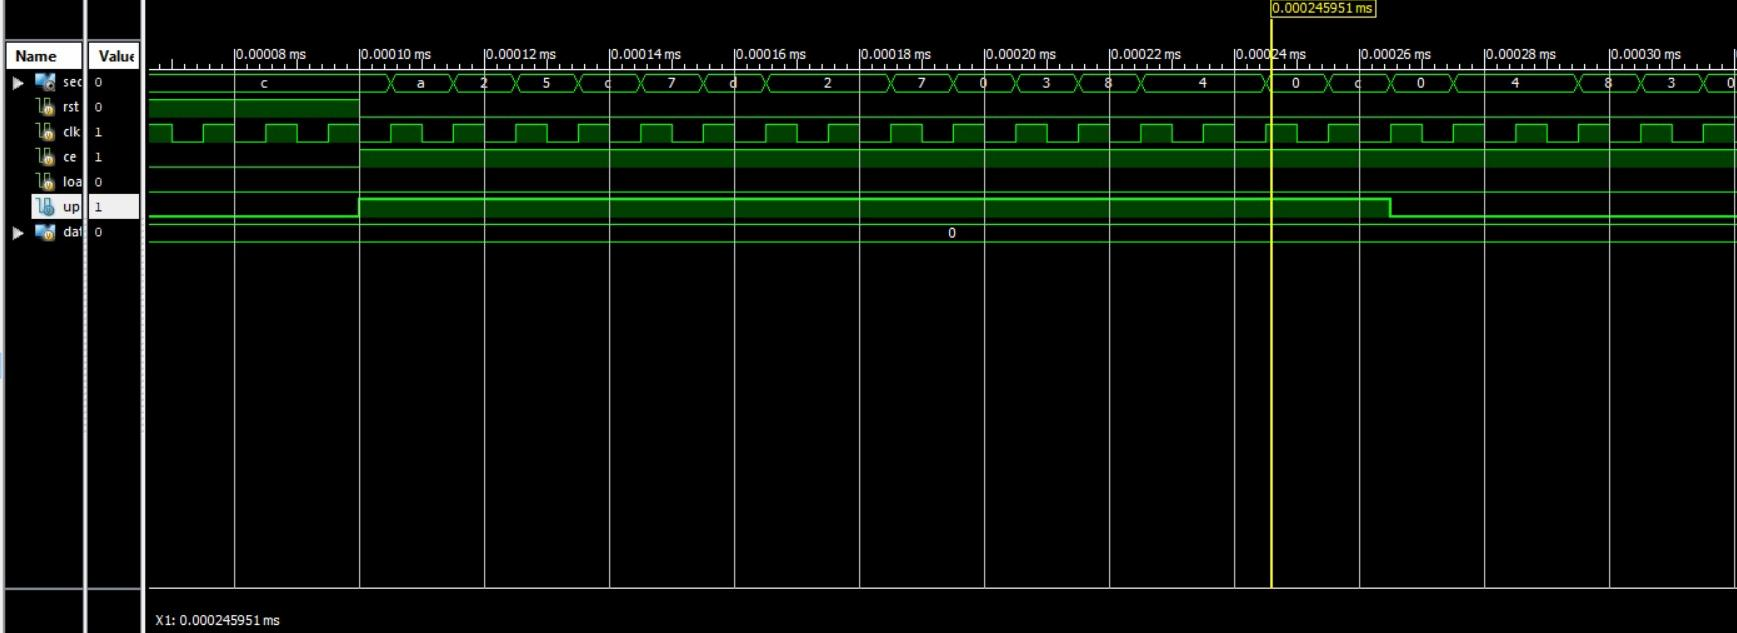
\includegraphics[width=\linewidth]{course-plis/images/lab2/test-result2.1}
	\caption{Реализация цифрового автомата. Часть 1}
	\label{fig:2isim1}
\end{figure}

\begin{figure}[h!]
	\centering
	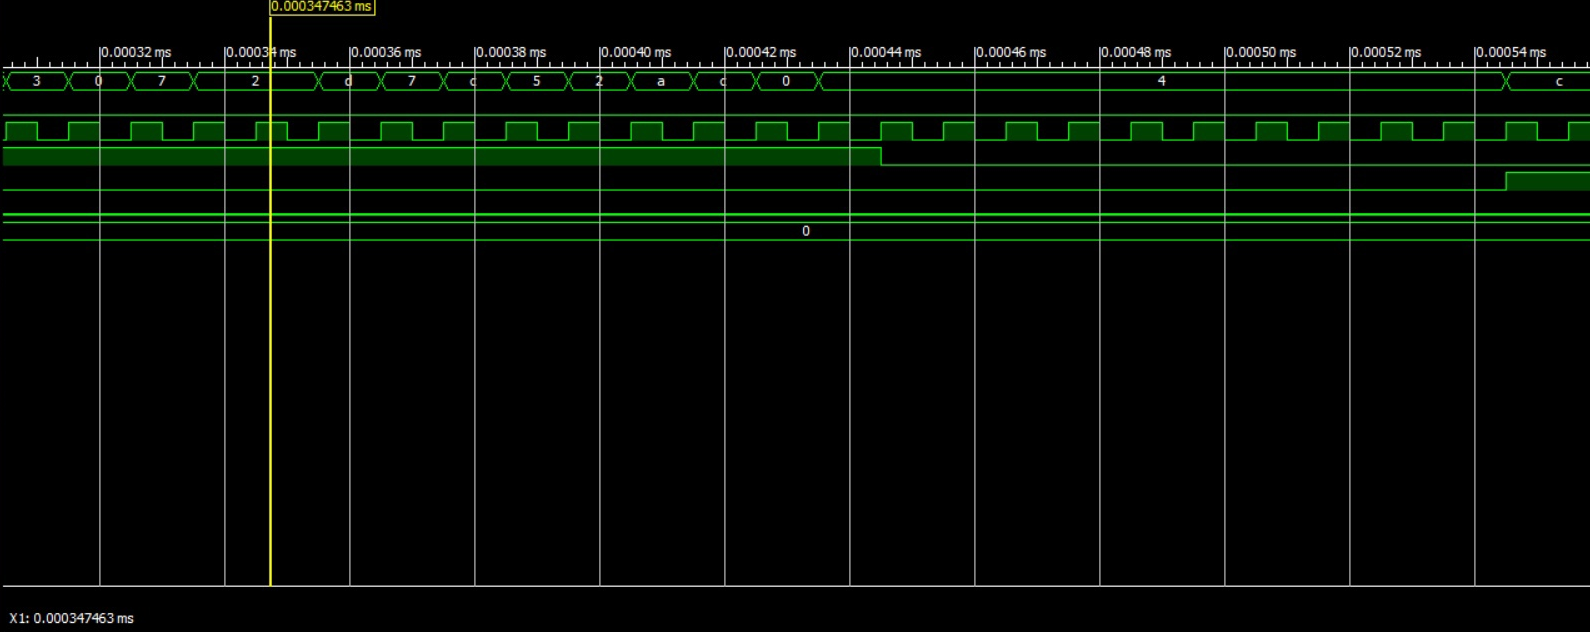
\includegraphics[width=\linewidth]{course-plis/images/lab2/test-result2.3}
	\caption{Реализация цифрового автомата. Часть 2}
	\label{fig:2isim2}
\end{figure}





% Lab3 

% TODO: \usepackage{graphicx} required
\begin{figure}[h!]
	\centering
	\includegraphics[width=1\linewidth]{course-plis/images/lab3/page-1}
	\caption{Реализация анализатора последовательности. Часть 1}
	\label{fig:3page-1}
\end{figure}
% TODO: \usepackage{graphicx} required
\begin{figure}[h!]
	\includegraphics[width=1\linewidth]{course-plis/images/lab3/page-2}
\caption{Реализация анализатора последовательности. Часть 2}
	\label{fig:3page-2}
\end{figure}
% TODO: \usepackage{graphicx} required
\begin{figure}[h!]
	\centering
	\includegraphics[width=1\linewidth]{course-plis/images/lab3/page-3}
	\caption{Реализация анализатора последовательности. Часть 3}
	\label{fig:3page-3}
\end{figure}
% TODO: \usepackage{graphicx} required
\begin{figure}[h!]
	\centering
	\includegraphics[width=1\linewidth]{course-plis/images/lab3/page-4}
	\caption{Реализация анализатора последовательности. Часть 4}
	\label{fig:3page-4}
\end{figure}
% TODO: \usepackage{graphicx} required
\begin{figure}[h!]
	\centering
	\includegraphics[width=1\linewidth]{course-plis/images/lab3/page-5}
	\caption{Реализация анализатора последовательности. Часть 5}
	\label{fig:3page-5}
\end{figure}
% TODO: \usepackage{graphicx} required
\begin{figure}[h!]
	\centering
	\includegraphics[width=1\linewidth]{course-plis/images/lab3/page-6}
	\caption{Реализация анализатора последовательности. Часть 6}
	\label{fig:3page-6}
\end{figure}



%Lab 4
\begin{figure}[h!]
	\centering
	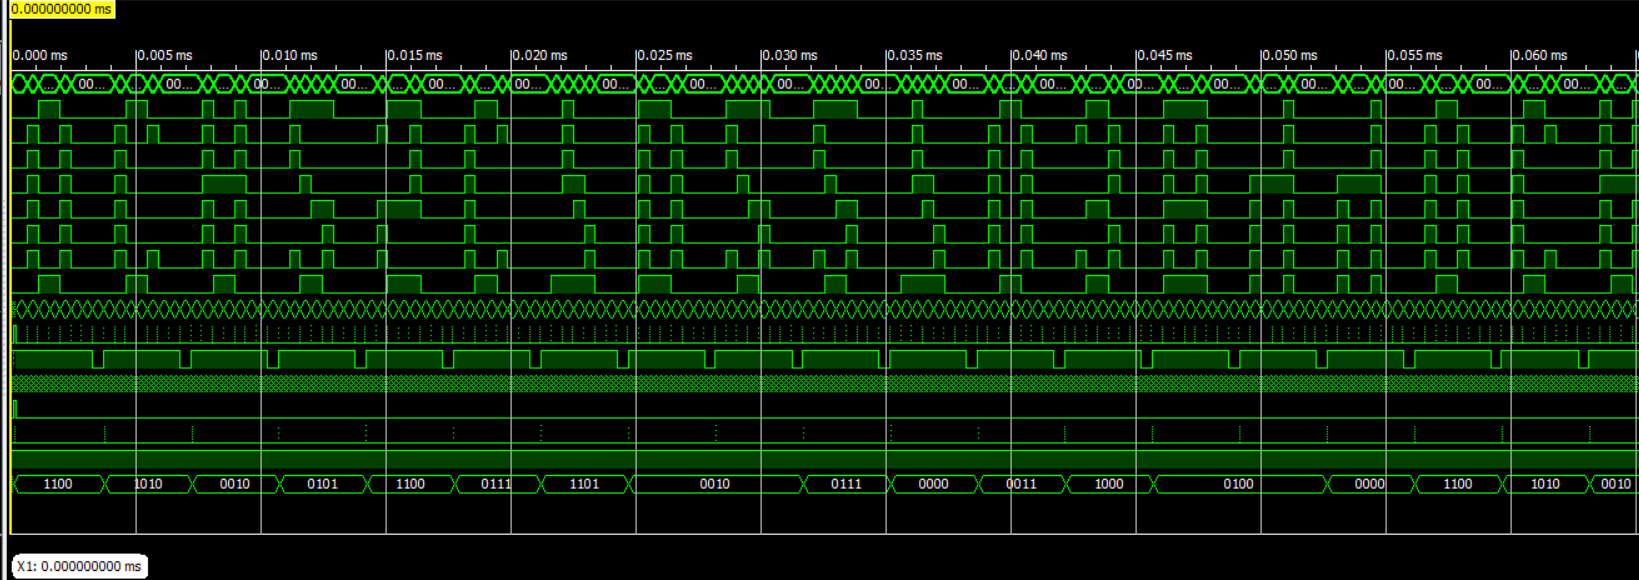
\includegraphics[width=1\linewidth]{course-plis/images/lab4/4isim}
	\caption{Управление матричным индикатором. Результат симуляции}
	\label{fig:4isim}
\end{figure}



%Lab5
\begin{figure}[h!]
	\centering
	\includegraphics[width=1\linewidth]{course-plis/images/lab5/isim1}
	\caption{Генерация ШИМ. Результат симуляции. Часть 1}
	\label{fig:5isim1}
\end{figure}

\begin{figure}[t!]
	\centering
	\includegraphics[width=1\linewidth]{course-plis/images/lab5/isim2}
	\caption{Генерация ШИМ. Результат симуляции. Часть 2}
	\label{fig:5isim2}
\end{figure}

%\vspace{50ex}
%\vfill




%\begin{lstlisting}[style=pseudocode,caption={Алгоритм оценки дипломных работ}]
%	sdfsadf sdf asdf sadf s
%\end{lstlisting}
%%% Local Variables: 
%%% mode: latex
%%% TeX-master: "rpz"
%%% End: 
